% !TeX root = ../main.tex

\section{X-ray diffraction}

\begin{problem}[Structure factor for a tri-atomic basis]
  Consider a linear crystal with lattice constant $a$ in which the basis
  consists of atom of species $A$ at $0$ and two atoms of species $B$ at $1/3$
  and $2/3$.
  \begin{enumext}
    \item Find the structure factor of such a crystal.
    \item X-rays of wavelength $\lambda (= a/4)$ irradiate this crystal at an
    oblique incidence ($\qty{45}\degree$). Using the Ewald construction in the
    plane of incidence, show graphically, the diffraction directions and
    indicate the relative weights of the different diffracted intensities.
    \item State the physical significance of the vector $\bm k$ from which the
    extremity is on a plane passing through the origin of the reciprocal lattice.
  \end{enumext}
\end{problem}
\begin{solution}[By TA]
  \begin{enumext}
    \item \[
      S_a = \sum_j f_j \upe^{-\iu \bm a \cdot \bm r_j}
    = f_A \upe^{-\iu\bm G\cdot0} + f_B(\upe^{-\iu\bm G\cdot\frac a3\hat x}
    + \upe^{-\iu\bm a\cdot\frac23 a\hat x})
    = f_A + 2f_B\cos(\frac{2\pi}{3}h)
    = \begin{cases}
      f_A + 2f_B,\\
      f_A - f_B
    \end{cases}
    \]
    \item $k = \frac{2\pi}{\lambda} = \frac{8\pi}{a}$,
    \[
      k\cos\qty{45}\degree - k\cos\theta = G_x
    \]
    $\cos\theta = \frac{h + 2\sqrt2}{4} \in [-1, 1]$.
  \end{enumext}
\end{solution}
\begin{solution}\leavevmode
  \begin{enumext}
    \item Substitute $r_i = 0$, $\frac a3$, $\frac{2a}3$ into the definition of
    the structure factor
    \begin{align*}
    S(h) & = f_A\upe^{\iu G\cdot 0} + f_B\upe^{\iu G\cdot\frac a3}
           + f_B\upe^{\iu G\cdot\frac{2a}{3}}
      \xlongequal{G = 2\pi h/a} f_A + f_B
             \ab(\upe^{\iu\frac{2\pi h}{3}} + \upe^{\iu\frac{4\pi h}{3}})\\
    & \xlongequal{\text{Euler's formula}}
    \begin{cases}
      f_A + 2f_B, & h = 3n\\
      f_A - f_B,  & \text{otherwise}
    \end{cases}
    \end{align*}
    \item The wave number
    \[
      k = \frac{2\pi}{\lambda} = \frac{8\pi}{a} = 4b_0,
    \]
    where $b_0 = \frac{2\pi}{a}$ is the reciprocal lattice vector.
    The incident wavevector is
    \[
      \bm k_i = \ab(k/\sqrt2, -k/\sqrt 2)
    \]
    \begin{paracol}{2}
    Then, the Ewald circle satisfies
    \[
      \ab(x + k/\sqrt2)^2 + \ab(y - k/\sqrt2)^2 = k^2
    \]
    and we can obtain the two intersection on $x$-axis: $x_1 = 0$ and
    $x_1 = -\sqrt2k$.

    Obviously, $x_1 = 0b_0$, $n_1 = 0$;
    $x_2 = -5.656b_0$, $n_2 = -5.656$.
    \switchcolumn \centering
    \vspace*\fill
    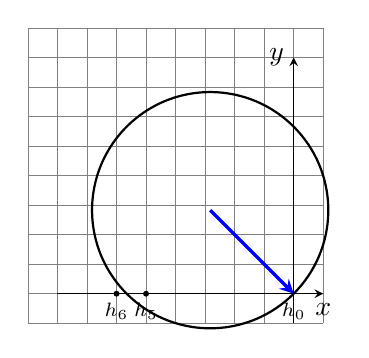
\begin{tikzpicture}[scale = .75]
      \draw [help lines, step = .5cm] (-4.5,4.5) grid (.5,-.5);
      \draw [-stealth] (-4,0) -- (.5,0) node [below] {$x$};
      \draw [-stealth] (0,-.5) -- (0,4) node [left] {$y$};
      \draw [thick] ({-2/sqrt(2)}, {2/sqrt(2)}) circle (2);
      \draw [blue, very thick, -stealth] ({-2/sqrt(2)}, {2/sqrt(2)}) -- (0,0);
      \fill (-2.5,0) circle (.05) (-3,0) circle (.05);
      \node [below] at (0,0) {$\scriptstyle h_0$};
      \node [below] at (-2.5,0) {$\scriptstyle h_5$};
      \node [below] at (-3,0) {$\scriptstyle h_6$};
    \end{tikzpicture}
    \vspace*\fill
    \end{paracol}
    Since $n$ is not an integer, no other reciprocal lattice points lies on the
    Ewald circle except the one on the original point.
    The intensity of each diffraction order is proportional to $|S(h)|^2$, i.e.,
    \[
      I_h \propto |S(h)|^2 =
      \begin{cases}
        (f_A + 2f_B)^2, & h = 3m,\\
        (f_A - f_B)^2,  & \text{otherwise}
      \end{cases}
    \]
    \item The tip of $\bm k$ lying on a plane through the origin of the
    reciprocal lattice means the Bragg condition is satisfied for diffraction.
  \end{enumext}
\end{solution}

\begin{problem}
  The main experimental methods of X-ray diffraction are
  \begin{enumext*}[label = (\alph*), columns = 2]
    \item the Laue method
    \item the crystal rotation method
    \item(2) the powder method (or the Debye-Scherrer method)
  \end{enumext*}
  Describe the corresponding experimental set-up and with the help of the Ewald
  construction in reciprocal space, deduce the observed diffraction patterns in
  each case.
\end{problem}
\begin{solution}\leavevmode
  \begin{enumext}
    \item Laue Method
    \begin{enumext}
      \item Setup: Stationary single crystal, polychromatic X-rays.
      \item Ewald \& Pattern: A continuous range of Ewald sphere radii (due to
      varying $\lambda$) means many reciprocal lattice points lie on some
      sphere. This produces a pattern of sharp spots, each from a different
      $(hkl)$ plane and wavelength. The spot arrangement directly reveals the
      crystal's symmetry.
    \end{enumext}
    \item Crystal Rotation Method
    \begin{enumext}
      \item Setup: Rotating single crystal, monochromatic X-rays.
      \item Ewald \& Pattern: The fixed Ewald sphere is intersected by rotating
      reciprocal lattice points. This generates discrete spots or arcs on the
      detector. Measuring the rotation angles and intensities of these spots
      allows for the determination of the unit cell and atomic structure.
    \end{enumext}
    \item Powder Method
    \begin{enumext}
      \item Setup: Powdered sample (random crystallites), monochromatic X-rays.
      \item Ewald \& Pattern: Each set of $(hkl)$ planes forms a spherical shell
      in reciprocal space. The Ewald sphere's intersection with these shells
      creates cones of diffracted beams (Debye cones), which appear as
      characteristic rings on the detector. The ring positions
      ($2\theta$ angles) provide $d$-spacings for phase identification and
      lattice parameter calculation.
    \end{enumext}
  \end{enumext}
\end{solution}